%%%%%%%% Klassen-Optionen
\documentclass[12pt,a4paper]{scrartcl}

%%%%%%%% PAKETE: unverzichtbare Pakete mit Einstellungen
\usepackage[left=2.5cm, right=2cm, top=3cm, bottom=3cm, a4paper]{geometry} %Seitenrände
\usepackage[utf8x]{inputenc} % utf8-Kodierung und direkte Eingabe von Sonderzeichen
\usepackage{fixltx2e} % Verbessert einige Kernkompetenzen von LaTeX2e

%%%%%%%% PAKETE: AMS-Pakete
\usepackage{amsmath} % Mathe-Erweiterung
\usepackage{amsfonts} % Schrift-Erweiterung
\usepackage{amssymb} % Sonderzeichen-Erweiterung

%%%%%%%% PAKETE: Sonstiges
\usepackage[colorlinks, citecolor=black, filecolor=black, linkcolor=black, urlcolor=black]{hyperref} % Links
\usepackage{wrapfig} % ausgeklügekte Floatumgebung
\usepackage{float} % normale Floatumgebung
\restylefloat{figure} % ermöglicht die Verwendung von "H" (ist noch stärker als "h!")
\usepackage[small,it,singlelinecheck=false]{caption} % Bildunterschriften formatieren
\usepackage{multirow} % ermöglich Verbinden von Tabellenzeilen
\usepackage{multicol} % ermöglicht Spalten
\usepackage{fancyhdr} % ermöglicht Kopf- und Fußzeilen
\usepackage{graphicx} % Einbinden von Bildern möglich
\usepackage{units} % Einheiten
\usepackage{subcaption}

%%%%%%%% DEFINITIONEN: Titelseite
\author{April Cooper, Patrick Kreissl und Sebastian Weber}
\title{Worksheet 4: Error Analysis and Langevin
Thermostat}
\publishers{University of Stuttgart}
\date{\today}

%%%%%%%% ANPASSUNGEN: Kopf-und Fußzeile
\fancypagestyle{plain}{} % redefine the plain pagestyle to match the fancy layout
\pagestyle{fancy} % aktiviere eigenen Seitenstil
\fancyhf{} % alle Kopf- und Fußzeilen bereinigen
\fancyhead[L]{Worksheet 4: Error Analysis and Langevin
Thermostat
}
\fancyhead[R]{\today}
\renewcommand{\headrulewidth}{0.6pt} % obere Trennlinie
\fancyfoot[L]{April Cooper, Patrick Kreissl und Sebastian Weber}
\fancyfoot[R]{Page \thepage}
\renewcommand{\footrulewidth}{0.6pt} % untere Trennlinie

%%%%%%%% ANPASSUNGEN: Absätze
\setlength{\parindent}{0em} % keine Absatzeinzüge
\setlength{\parskip}{0em} % Absatz-Abstand

%%%%%%%% ANPASSUNGEN: Abbildungsverzeichnis
\usepackage{tocloft} % Zum Anpassen der Verzeichnisse
\renewcommand{\cftfigpresnum}{Abb. }
\renewcommand{\cfttabpresnum}{Tab. }
\renewcommand{\cftfigaftersnum}{:}
\renewcommand{\cfttabaftersnum}{:}
\setlength{\cftfignumwidth}{2cm}
\setlength{\cfttabnumwidth}{2cm}
\setlength{\cftfigindent}{0cm}
\setlength{\cfttabindent}{0cm}

%%%%%%%% SONSTIGES
\usepackage{pdfpages}
\usepackage{pgf}

% NÜTZLICH: http://truben.no/latex/table/

% Anfang des eigentlichen Dokuments
\begin{document}

\maketitle
\tableofcontents
\newpage

% =============== Section ============
\section{Error Analysis}
\subsection{Autocorrelation Analysis}
In this section we had to implement a Python function that computes the autocorrelaton function of a given time series and use this function on the given datasets. The resulting plot can be seen below:

%\begin{figure}[H]
%	\resizebox{1\textwidth}{!}{\input{../plots/acfplot.pdf}}
%	\caption{This plot shows the computed autocorrelation function of the given datasets.}
%	\label{fig:acfplot}
%\end{figure}

\begin{minipage}[hbt]{15cm}
	\centering
	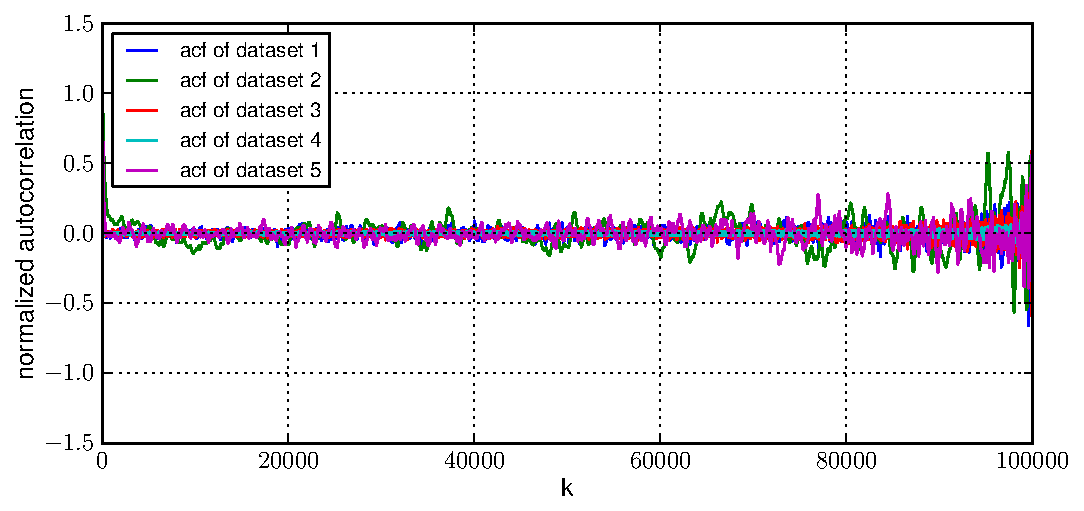
\includegraphics[width=16cm]{../plots/acfplot.pdf}
	%\caption{Bild1}
	%\label{fig:Bild1}
\end{minipage}

Furthermore we were supposed to plot the integrated autocorrelation function which can be seen below:

\begin{minipage}[hbt]{15cm}
	\centering
	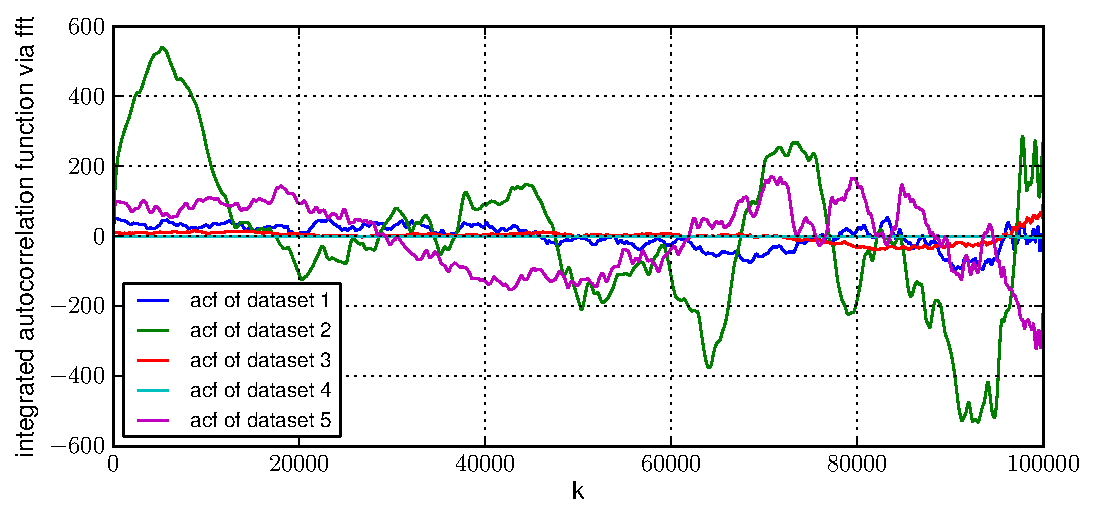
\includegraphics[width=16cm]{../plots/acfintplot.pdf}
	%\caption{Bild1}
	%\label{fig:Bild1}
\end{minipage}

As you can see in the plots, it is not useful to integrate the function over the whole interval because the lager the autocorellations shift parameter $k$ becomes the lareger the fluctuation of the autocorrelation function becomes. This is because for  larger $k$s due to the autocorrelations definition less data is used to compute the function. Therefore the statistical fluctuation of a single datapoint has more influence on the computed autocorrelation function. This larger fluctuation influences also manifest in the integrated autocorrelation function.
The integrated function should converge against the autocorrelation time. So for a visual estimate of the autocorrelation time the only relevant part of the interval is the one in which the autocorrelation funcion approximately acts like an exponetial function and where the influence of the intrisic error of the function due to the increased influence of statistical fluctuations is still relatively small. In the following plots we zoomed in to the relevant interval:

\begin{minipage}[hbt]{15cm}
	\centering
	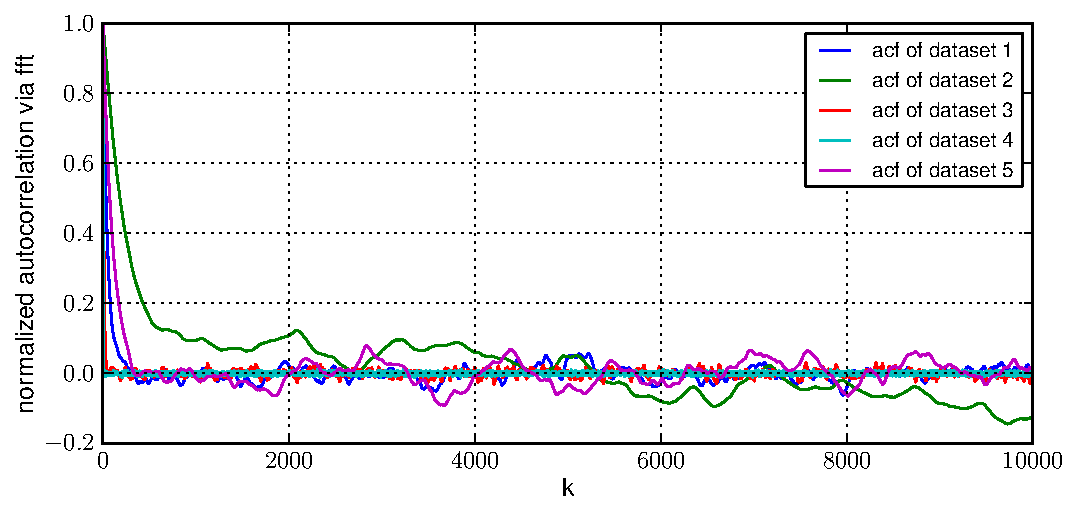
\includegraphics[width=16cm]{../plots/acfzoom.pdf}
	%\caption{Bild1}
	%\label{fig:Bild1}
\end{minipage}

\begin{minipage}[hbt]{15cm}
	\centering
	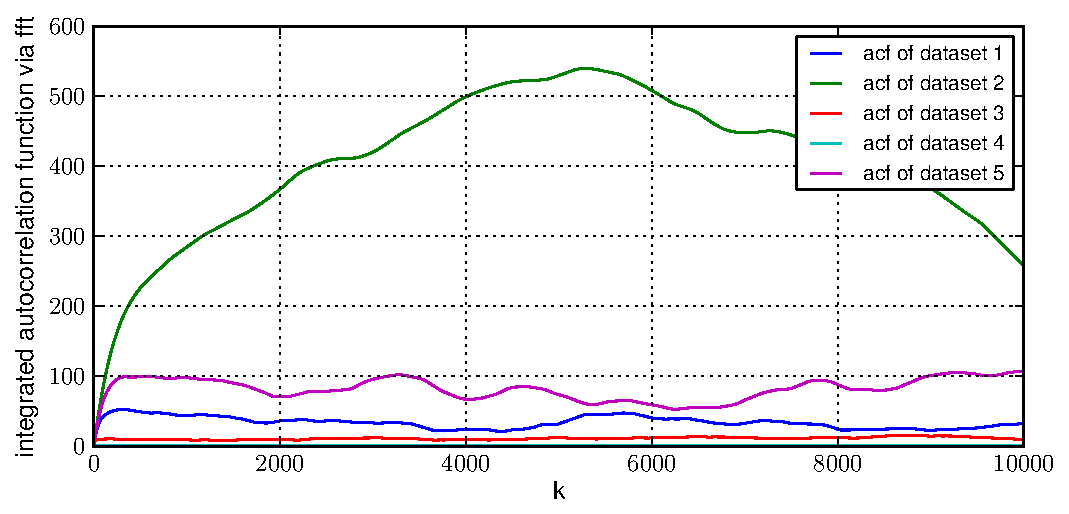
\includegraphics[width=16cm]{../plots/acfintzoom.pdf}
	%\caption{Bild1}
	%\label{fig:Bild1}
\end{minipage}

The autocorrelation times of the datasets can be visually guessed as follows:

\begin{center}
\begin{tabular}{|c|c|}
\hline 
dataset & guessed autocorrelation time \\ 
\hline 
1 & 50 \\ 
\hline 
2 & 450 \\ 
\hline 
3 & 10 \\ 
\hline 
4 & 1 \\ 
\hline 
5 & 90 \\ 
\hline 
\end{tabular} 
\end{center}

The next task was to implement a Python function that performs automatic error analysis via autocorrelation analysis of a given time series of an observable.
This function should compute an estimate of the outocorrelation time via the running autocorrelation time estimator, where the integration is cut of when $k_\text{max} \geq 6 \hat{\tau}_{\cal{O},\text{int}}(k_\text{max})$.
The function was supposed to return the mean value of the observable $\bar{\cal O} {}$, the error of the mean value $\epsilon_{\bar{\cal O} {}}$, the estimated autocorrelation time $\hat{\tau}_{\cal{O},\text{int}}$, its error $\epsilon_{\hat{\tau}_{\cal{O},\text{int}}}$ and the effective statistics $N_\text{eff}$. The results shown in the folowing table:

\begin{center}
\begin{tabular}{|c|c|c|c|c|c|}
\hline 
dataset & $\bar{\cal O} {}$ & $\epsilon_{\bar{\cal O} {}}$ & $\hat{\tau}_{\cal{O},\text{int}}$ & $\epsilon_{\hat{\tau}_{\cal{O},\text{int}}}$ & $N_\text{eff}$ \\ 
\hline 
1 & $8.2468\cdot 10^{-15}$ & 0.0031 &  52.134 & 5.8381 & 956 \\ 
\hline 
2 & $3.9756 \cdot 10^{-14}$ & 0.0032 & 403.139 & 125.4145 & 123 \\ 
\hline 
3 & $4.0010 \cdot 10^{-15}$ & 0.0031 & 9.707 & 0.4736 & 5042 \\ 
\hline 
4 & $-1.4214 \cdot 10^{-13}$ & 0.0032 & 0.5039 & 0.0068 & 66666 \\ 
\hline 
5 & $-3.1724 \cdot 10^{-14}$ & 0.0032 & 99.4101 & 15.3684 & 502 \\ 
\hline 
\end{tabular} 
\end{center}

As you can see the visually estimated autocorrelation times are very similar to the computed ones. The dataset for witch it was most difficult to guess the autocorrelation time was dataset 2. This manifests in the computed error of the autocorrelation time of that dataset, too. It is nearly by factor 10 larger than the error of dataset 5, and even by factor 100 for the datasets 3 and 4.

\subsection{Binning Analysis}
We were supposed to implement a Python function that computes the block variance $\sigma^2_B$ for a given block size $k$. From that block variance the estimated autocorrelation time $\tau_{\cal{O},\text{int}}$ and error of the mean value $\epsilon_{\bar{\cal O} {}}$ can be computed. Our task was to plot theese for $1<k<2000$. The resulting plots are shown below:

\begin{minipage}[hbt]{15cm}
	\centering
	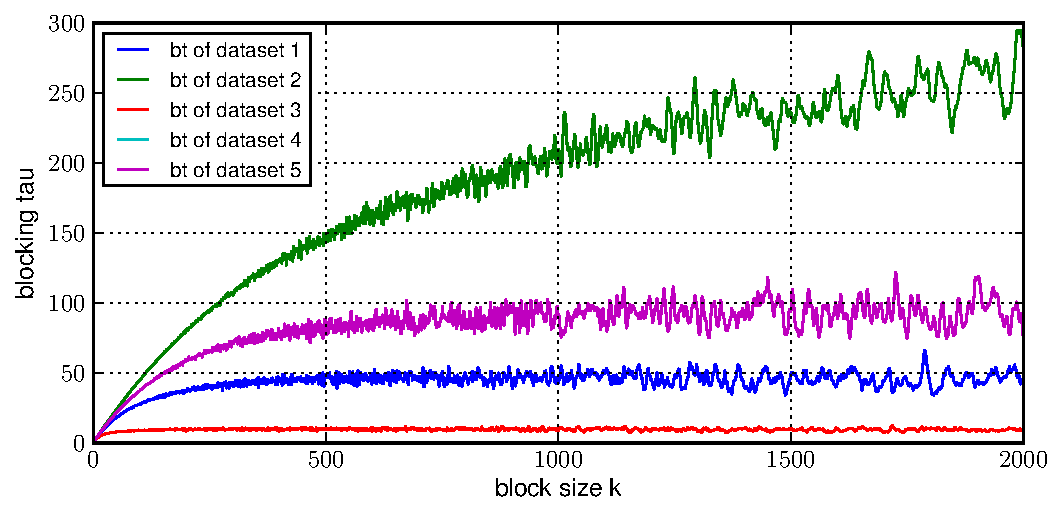
\includegraphics[width=16cm]{../plots/blockingtau.pdf}
	%\caption{Bild1}
	%\label{fig:Bild1}
\end{minipage}

\begin{minipage}[hbt]{15cm}
	\centering
	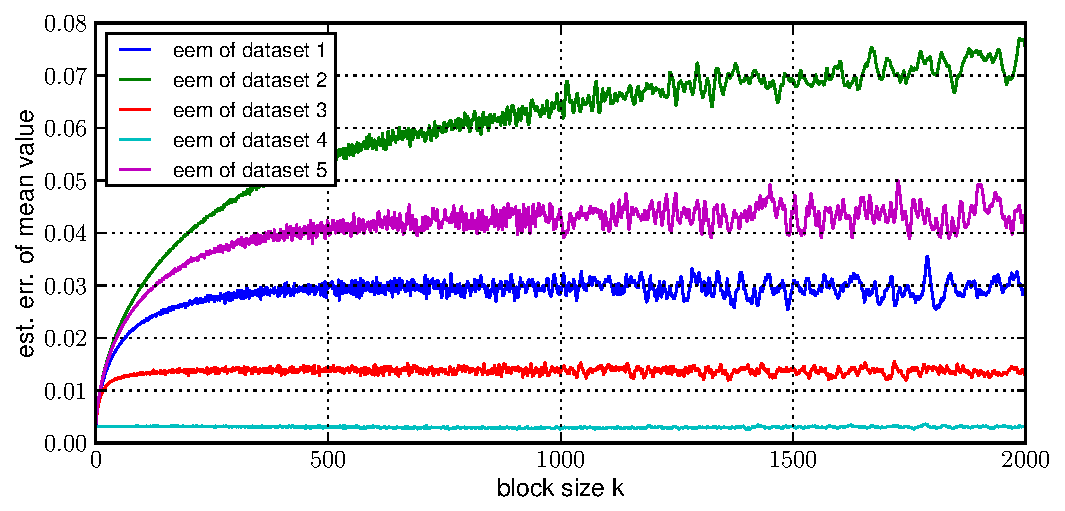
\includegraphics[width=16cm]{../plots/eem.pdf}
	%\caption{Bild1}
	%\label{fig:Bild1}
\end{minipage}

From the plots the autocorrelation time and the error of the mean value can be guessed as follows:

\begin{center}

\begin{tabular}{|c|c|c|}
\hline 
dataset & $\tau_{\cal{O},\text{int}}$ & $\epsilon_{\bar{\cal O} {}}$ \\ 
\hline 
1 & 49 & 0,030 \\ 
\hline 
2 & - & - \\ 
\hline 
3 & 10 & 0,014 \\ 
\hline 
4 & 1 & 0,004 \\ 
\hline 
5 & 90 & 0.042 \\ 
\hline 
\end{tabular} 

\end{center}

For both, autocorrelation time and the error of the mean value, for dataset 2 at the end of the interval ($k=2000$) the functions do still not converge, while the fluctuation of the data becomes already relatively large. Therefore for dataset 2 no values could be estimated.\\
For the others the autocorrelation time matches the values obtained in the previous tasks. For the error of the mean value only the error of dataset 1 matches the previous estimated value. The error of the other is smaller than previously obtained.

\subsection{Jackknife Analysis}
In this section we had to implement a Python funcion that computes the Jackknife error $\epsilon_{\bar{\cal O} {}}$ for a given time series and block size $k$. The resulting plot is shown below:

\begin{minipage}[hbt]{15cm}
	\centering
	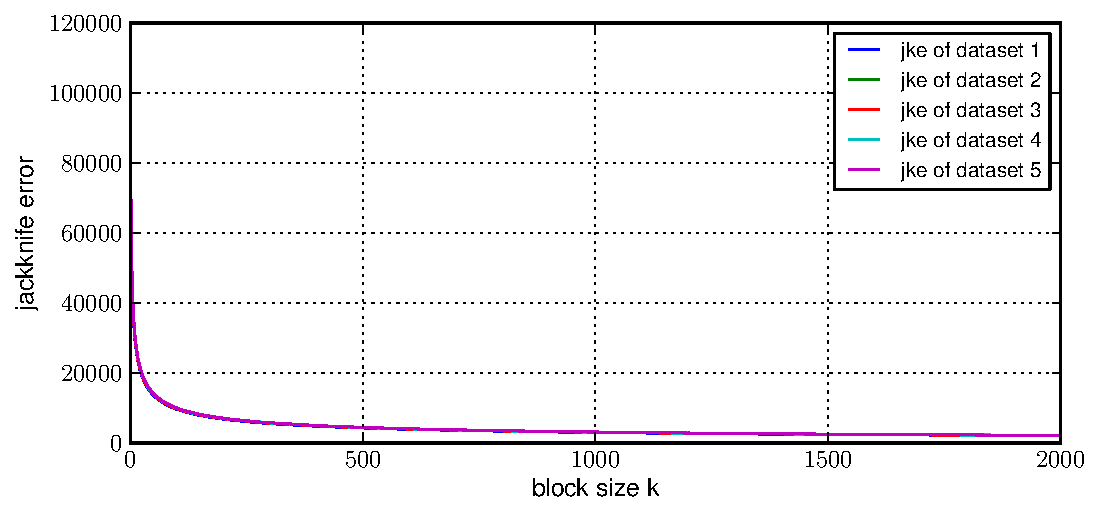
\includegraphics[width=16cm]{../plots/jackk.pdf}
	%\caption{Bild1}
	%\label{fig:Bild1}
\end{minipage}

The computed errors would range from 2126 to 2203 at $k=2000$. That seems hardly plausible and does not match the values obtained in the other tasks at all.

\end{document}


% =============== Comments ============
\begin{comment}
\verb{x_init {}}

\begin{figure}[H]
	\resizebox{1\textwidth}{!}{\input{../plots/NAME.pgf}}
	\caption{CAPTION}\label{fig:NAME}
\end{figure}
\end{comment}
